\subsection{Standard Signals}

\begin{figure}[h!]
\centering
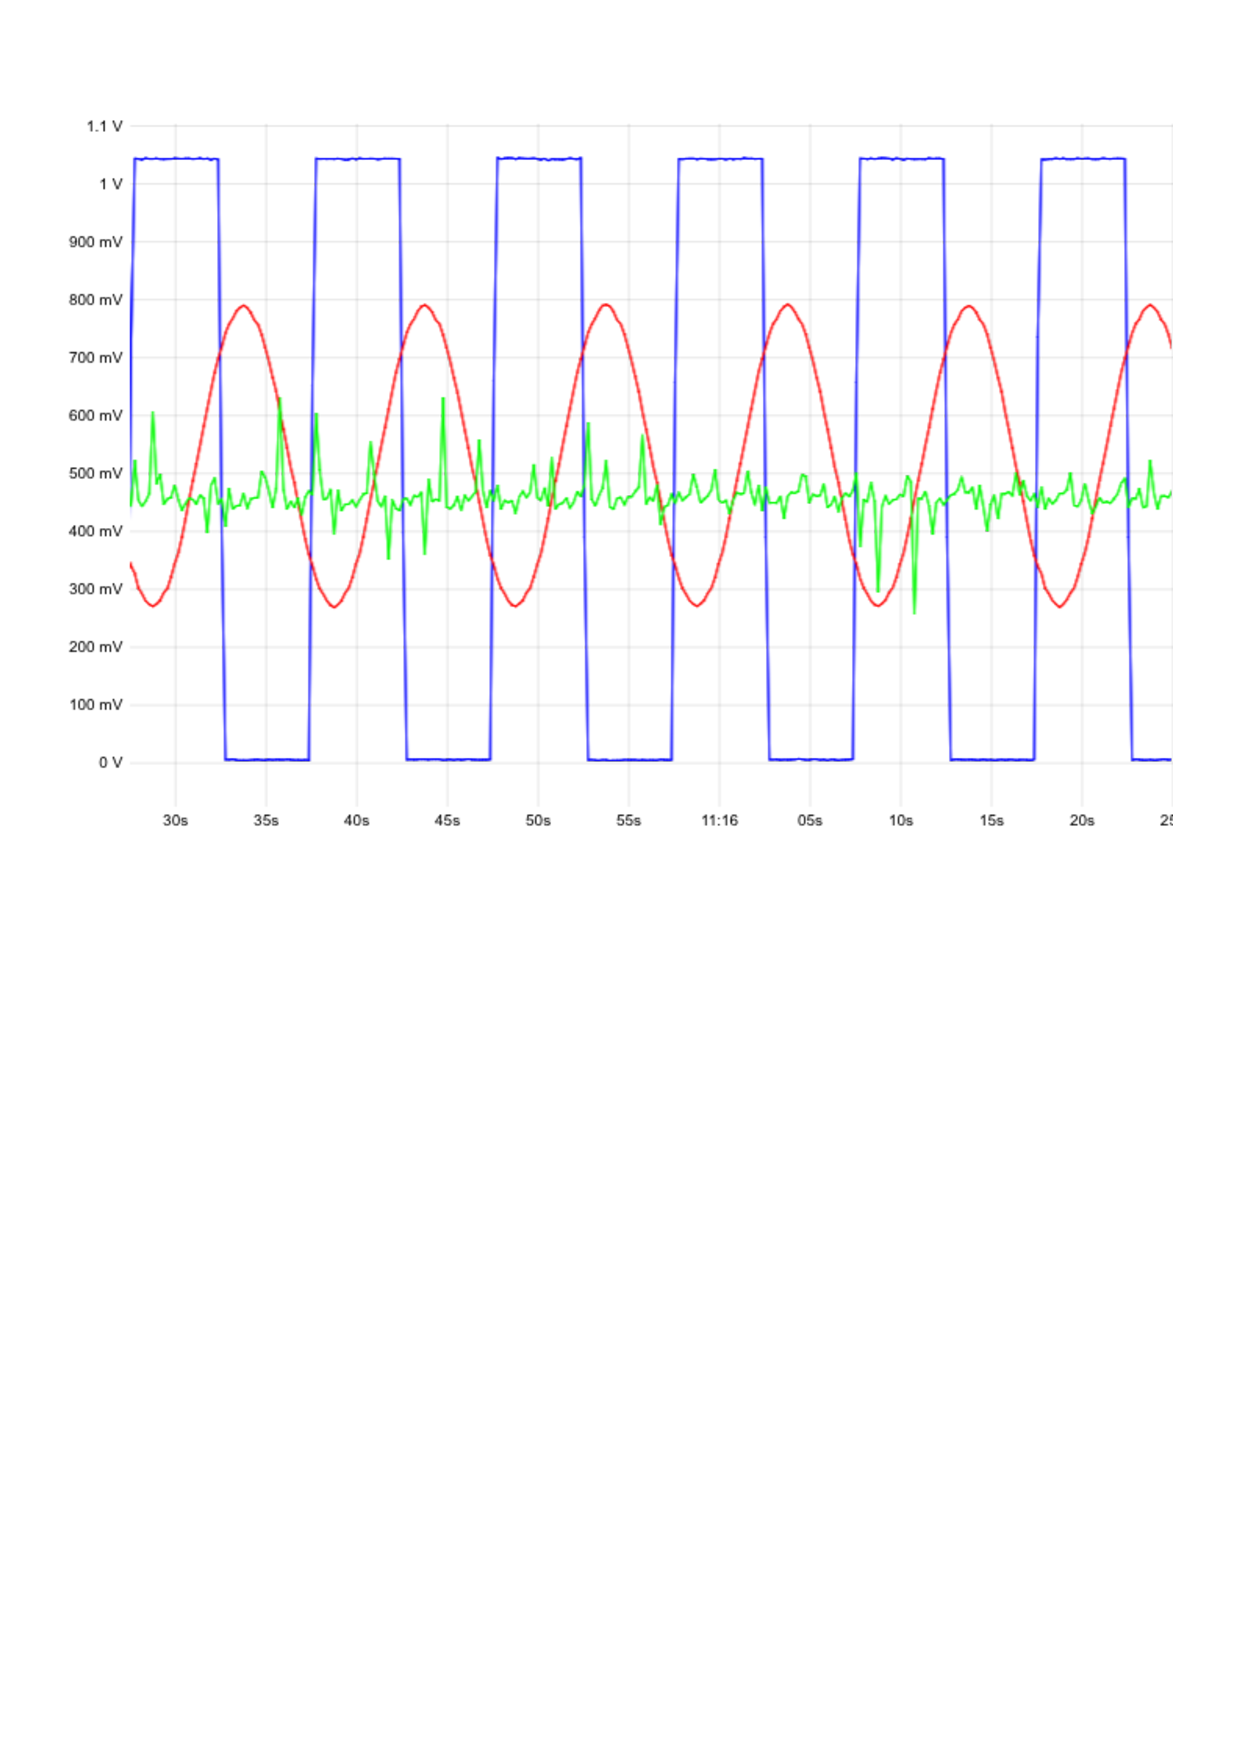
\includegraphics[trim={0cm 0cm 0cm  0cm}, clip, width=.75\textwidth]{./figures/standardsignals/picologChemComp.pdf}
\captionsetup{justification=centering}
\caption{Standard signals recorded using a PicoScope. Green: noise, red: sine wave, blue: square wave.}
\label{fig: test1 picolog}
\bigbreak
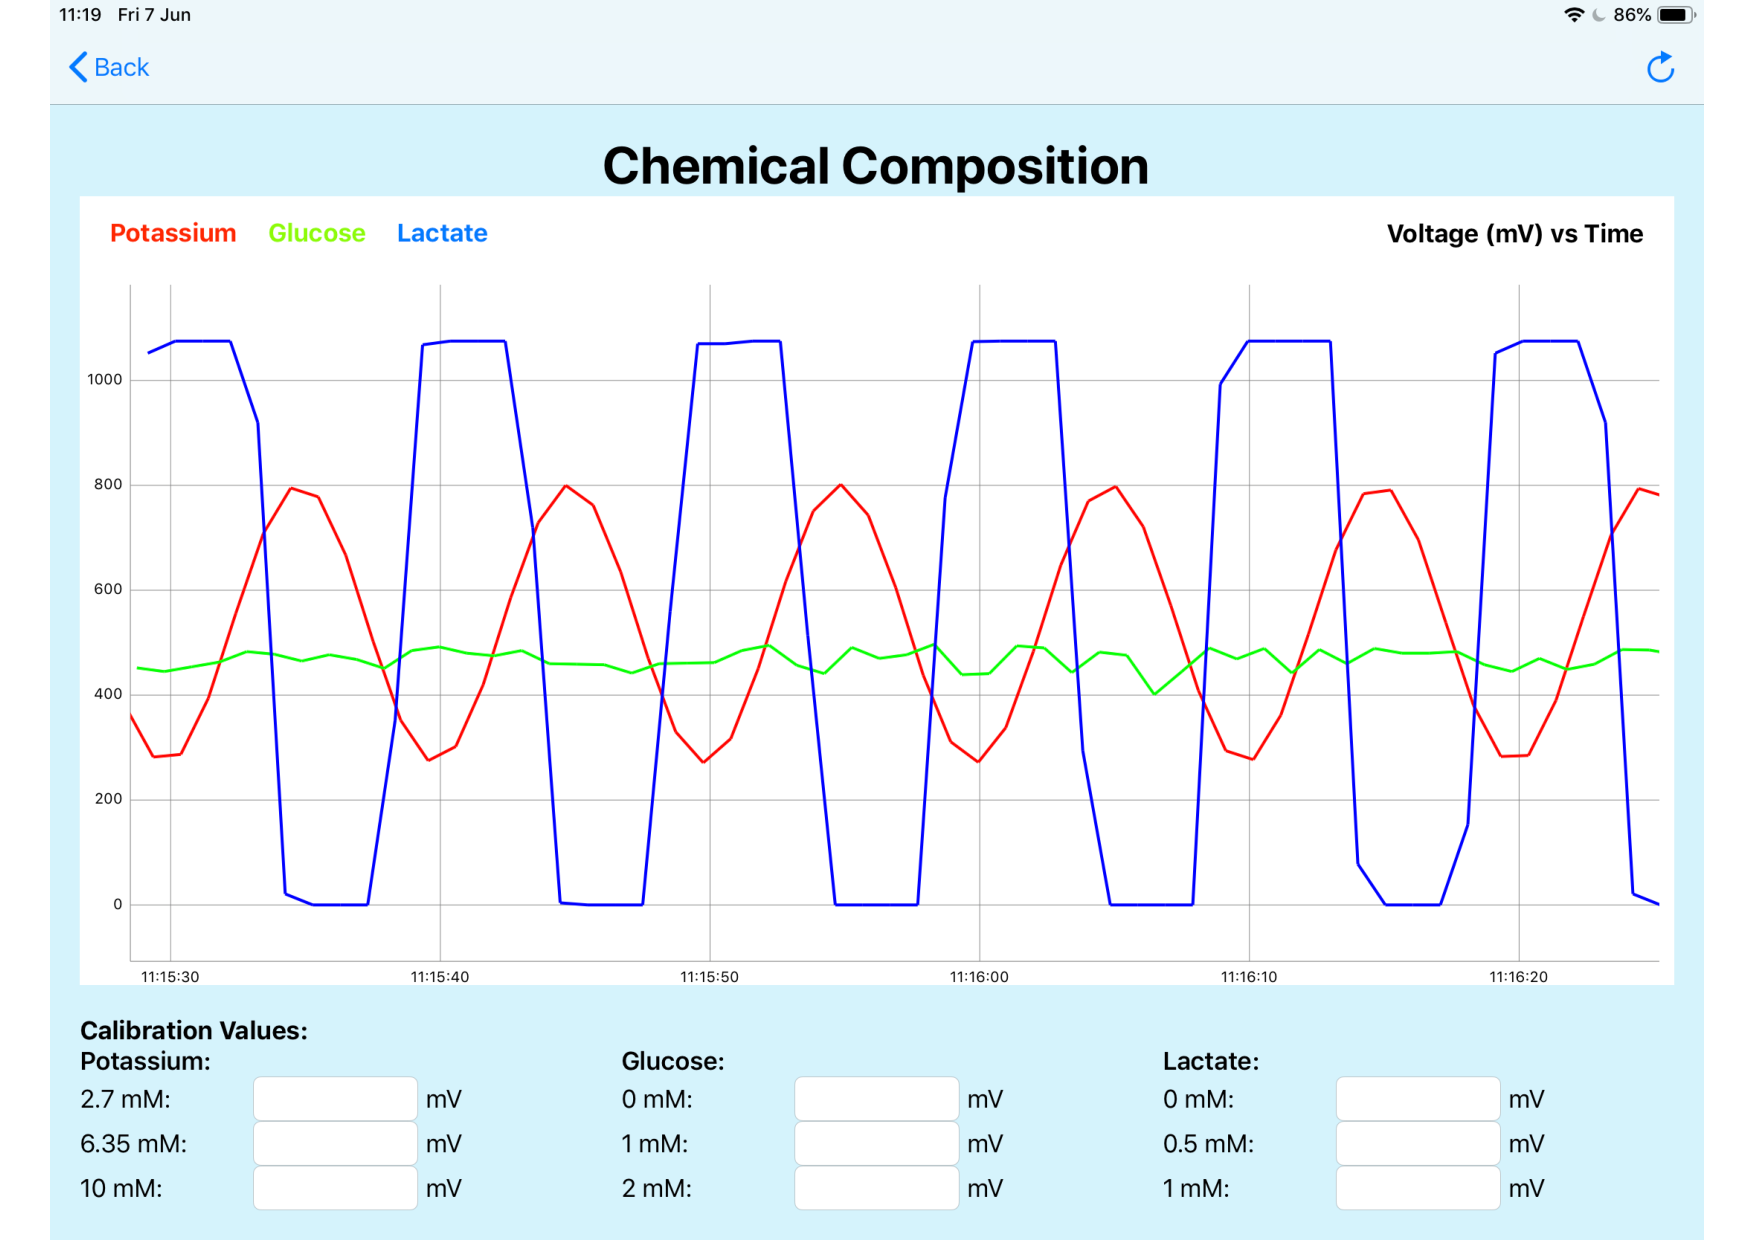
\includegraphics[trim={0cm 0cm 0cm  0cm}, clip, width=.75\textwidth]{./figures/standardsignals/appChemComp.pdf}
\captionsetup{justification=centering}
\caption{Standard signals recorded on iPad app. Green: noise, red: sine wave, blue: square wave.}
\label{fig: test1 app}
\end{figure}



Figure~\ref{fig: test1 picolog} shows the raw signals received on PicoLog, and Figure~\ref{fig: test1 app} shows the same three signals received on the Chemical Composition page of the app after undergoing filtering and processing on the Arduino.


\subsection{Spreading Depolarisation}

\begin{figure}[h!]
\centering
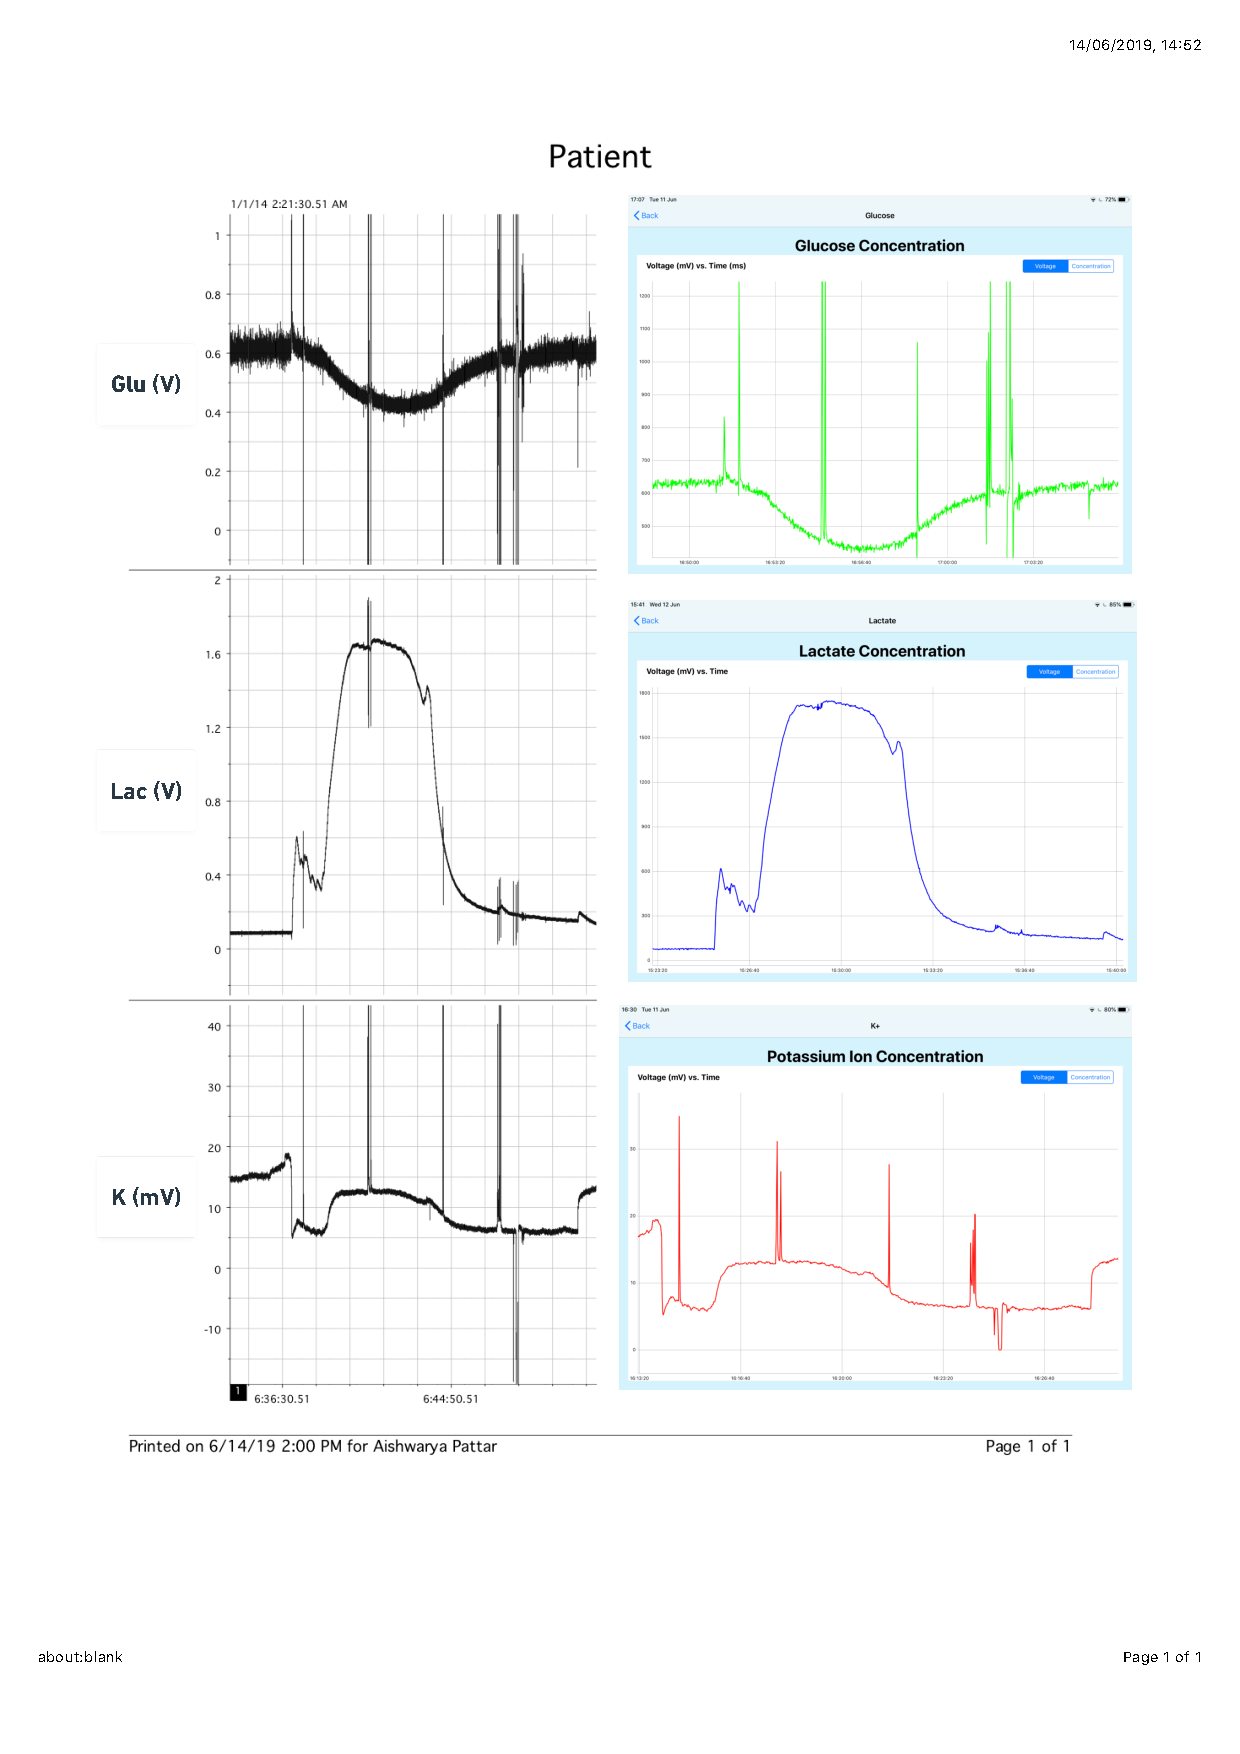
\includegraphics[trim={0cm 0cm 0cm  0cm}, clip, width=0.975\textwidth]{./figures/test2.pdf}
\captionsetup{justification=centering}
\caption{Left: Raw patient data. Right: Signals received on app. Top to bottom: Glucose, Lactate, Potassium. Plots of voltage against time.}
\label{fig: test2}
\end{figure}

Figure~\ref{fig: test2} shows the raw patient signals, before downsampling and processing, compared to the signals received on the app. Figure~\ref{fig: test2 conc} shows the concentration vs. time graphs produced on the app calculated from the inputted calibration values.

\begin{figure}[p]
\centering
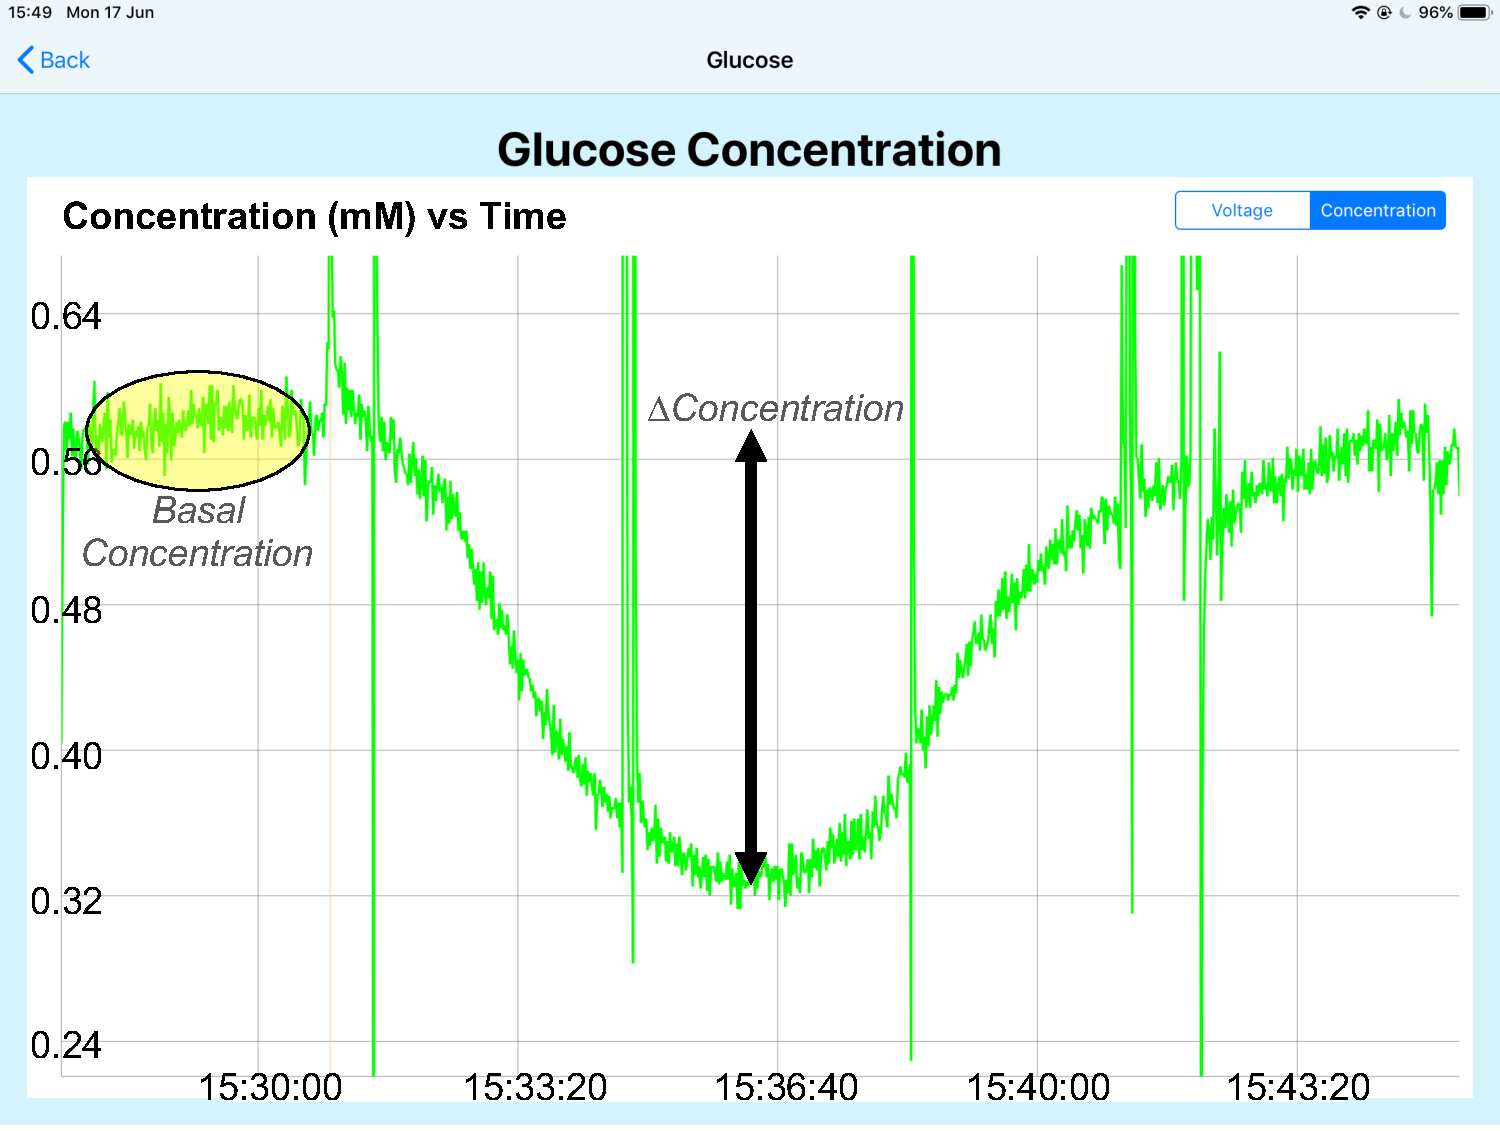
\includegraphics[trim={0cm 0cm 0cm  0cm}, clip, width=.6\textwidth]{./figures/patientsignals/Gconc.pdf}
\bigbreak
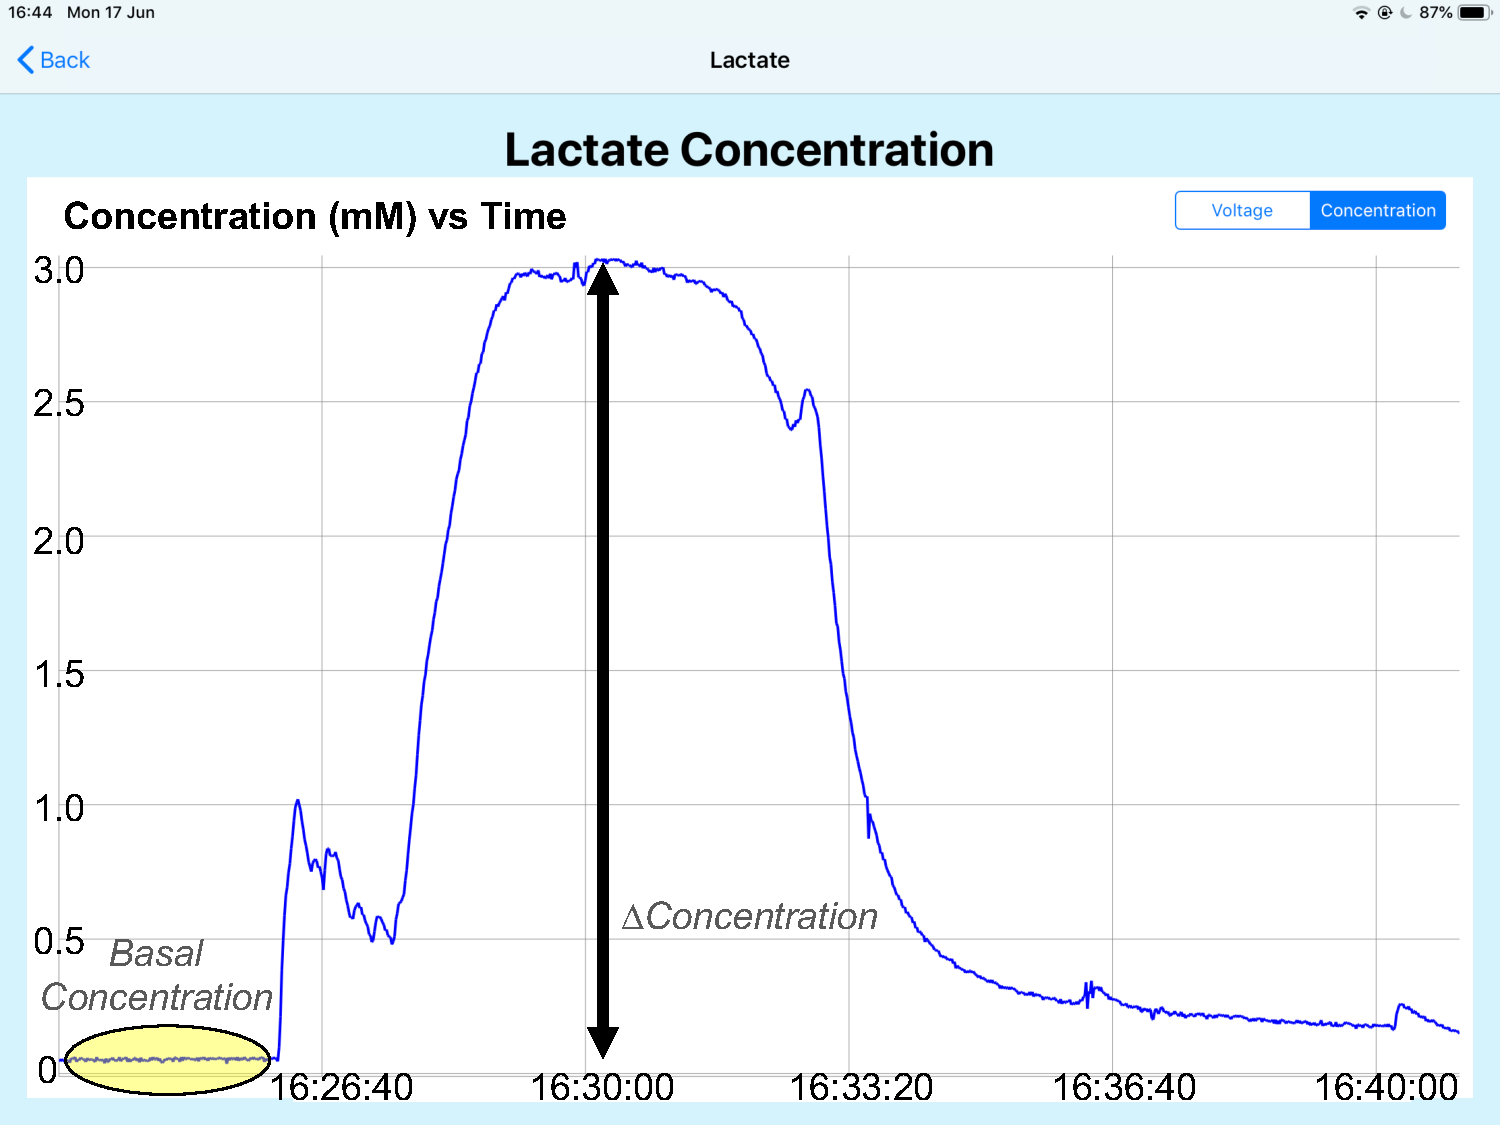
\includegraphics[trim={0cm 0cm 0cm  0cm}, clip, width=.6\textwidth]{./figures/patientsignals/Lconc.pdf}
\bigbreak
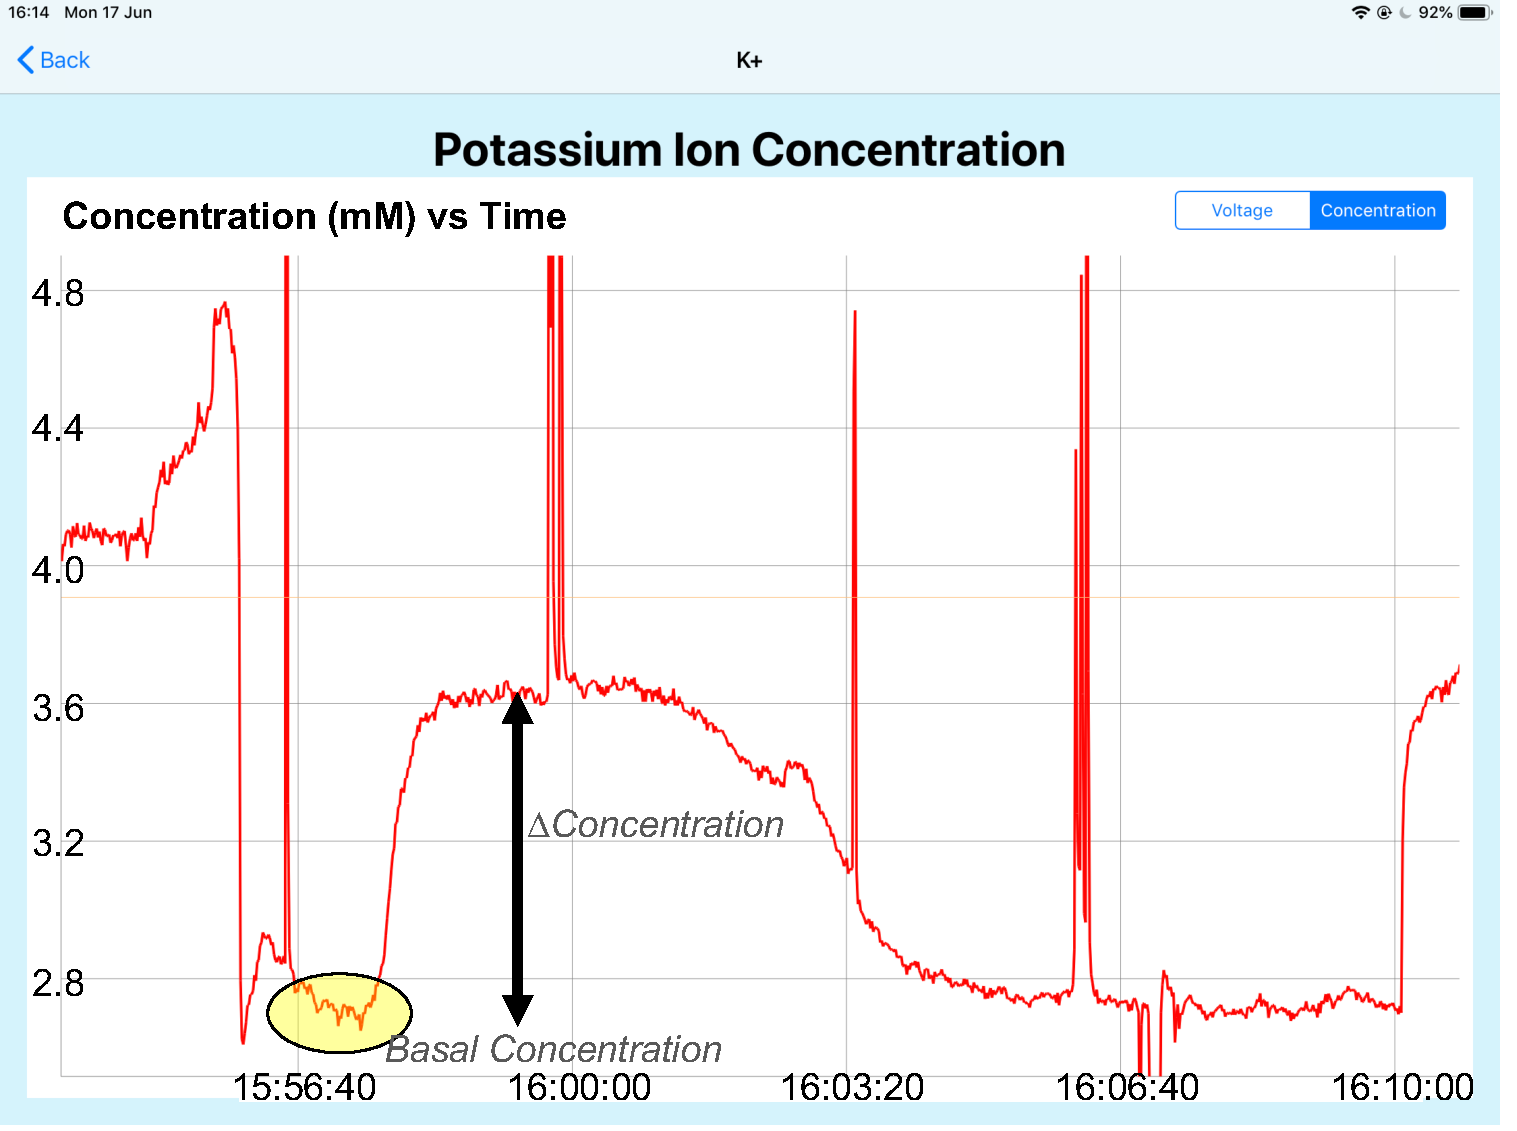
\includegraphics[trim={0cm 0cm 0cm  0cm}, clip, width=.6\textwidth]{./figures/patientsignals/Kconc.pdf}
\captionsetup{justification=centering}
\caption{Concentration (mM) vs. time graphs calculated from calibration values. Basal concentration and transient concentration change during an SD are shown.}
\label{fig: test2 conc}
\end{figure}